\documentclass[aspectratio=169,xcolor=dvipsnames]{beamer}
\usetheme{Simple}

\usepackage[utf8]{vietnam}
\usepackage{hyperref}
\usepackage{graphicx}
\usepackage{booktabs}
\usepackage{tikz, forest}

\usetikzlibrary{arrows.meta, shapes}
\forestset{
	.style={
		for tree={
			base=bottom,
			child anchor=north,
			s sep+=1cm,
			straight edge/.style={
				edge path={\noexpand\path[\forestoption{edge},thick,-{Latex}] 
					(!u.parent anchor) -- (.child anchor);}
			},
			if n children={0}
			{tier=word, draw, thick, rectangle}
			{draw, diamond, thick, aspect=2},
			if n=1{%
				edge path={\noexpand\path[\forestoption{edge},thick,-{Latex}] 
					(!u.parent anchor) -| (.child anchor) node[pos=.2, above] {Y};}
			}{
				edge path={\noexpand\path[\forestoption{edge},thick,-{Latex}] 
					(!u.parent anchor) -| (.child anchor) node[pos=.2, above] {N};}
			}
		}
	}
}

\usepackage[backend=biber]{biblatex}
\addbibresource{sample.bib}

\title[Fakenews Detection]{Ứng dụng Decision Tree xây dựng \\ công cụ Fakenews Detection}
\subtitle{Đồ án môn học Xử lý ngôn ngữ tự nhiên ứng dụng (CSC15008)}

\author[Quan-Tran] {Trần Hoàng Quân - Lê Hoàng Trọng Tín}

\institute[HCMUS]
{
    Khoa Công nghệ thông tin \\
    Trường Đại học Khoa học Tự nhiên - ĐHQG HCM
}
\date{\today}

\begin{document}

\begin{frame}
    \titlepage
\end{frame}

\begin{frame}{Nội dung}
    \tableofcontents
\end{frame}

\section{Giới thiệu}

\begin{frame}
	\Huge{\centerline{\textbf{Giới thiệu}}}
\end{frame}


\begin{frame}{Giới thiệu}
\begin{alertblock}{Nghe có vẻ \textbf{thật}, nhưng đây là \textbf{fake news}}
"Wikileaks released tonight a new cache of documents, showing that the United States  National Security Administration bugged private meetings between major world leaders, including the United Nations Secretary General.The N.S.A. bugged meetings between U.N.S.G. Ban Ki-Moon, German chancellor Angela Merkel, Italian prime minister Silvio Berlusconi, Israeli prime minister Benjamin Netanyahu, and several representatives from other major world governments, listening in on their conversations on climate change, global economics, and even  how to deal with Obama,  according to the new documents. "
\end{alertblock}
\end{frame}

\begin{frame}{Giới thiệu (cont.)}
\begin{itemize}
\item Tin giả (fakenews) đã trở thành chủ đề đáng quan tâm trong những năm gần đây.
\item Nhu cầu xây dựng công cụ xác minh tin giả (fakenews detector) trở nên cần thiết.
\item Có thể ứng dụng bài toán Text Classification xây dựng công cụ xác minh tin giả.
\begin{itemize}
    \item Gán nhãn một article là `0` nếu câu đó là tin giả, `1` nếu đó là tin thật.
\end{itemize}
\end{itemize}
\end{frame}

\section{Fakenews Detection}

\begin{frame}
	\Huge{\centerline{\textbf{Data}}}
\end{frame}

\subsection{Data}
\begin{frame}{Data}
Dataset gồm 44898 bài báo được thu thập trong năm 2017. \href{https://www.kaggle.com/datasets/clmentbisaillon/fake-and-real-news-dataset}{Link dataset trên Kaggle}
\begin{figure}
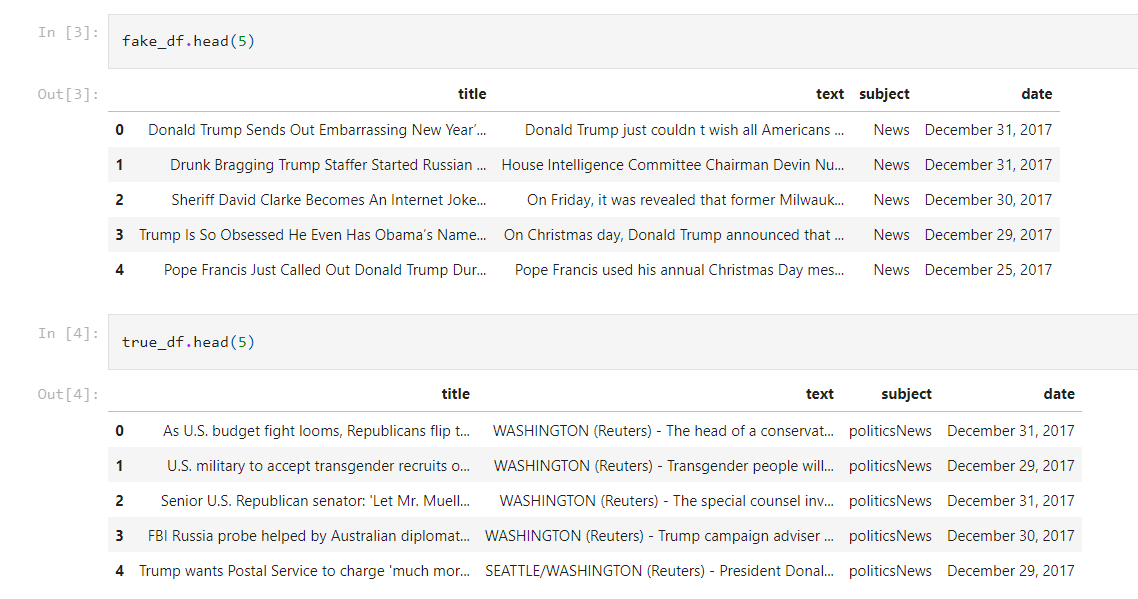
\includegraphics[width=0.8\linewidth]{img/quick-glance-at-data.PNG}
\end{figure}
\end{frame}


\begin{frame}
	\Huge{\centerline{\textbf{Preprocessing}}}
\end{frame}

\subsection{Preprocessing}
\begin{frame}{Preprocessing}
\begin{itemize}
\item Ta cần chỉnh sửa cấu trúc dataset:
\begin{itemize}
\item Loại bỏ các cột \texttt{title}, \texttt{subject} và \texttt{date}. Tạm thời ta không cần những cột này.
\item Thêm cột \texttt{class} để gán nhãn tin thật / tin giả.
\end{itemize}
\item Bước tiền xử lý:
\begin{itemize}
\item Loại bỏ dấu câu
\item Chuyển câu về dạng chữ thường
\item Loại bỏ số
\item Loại bỏ links, html tags và ký tự đặc biệt
\item Loại bỏ stopwords
\end{itemize}
\end{itemize}
\end{frame}

\begin{frame}{Preprocessing (cont.)}
\begin{columns}[c]
\column{.5\textwidth}
\begin{figure}
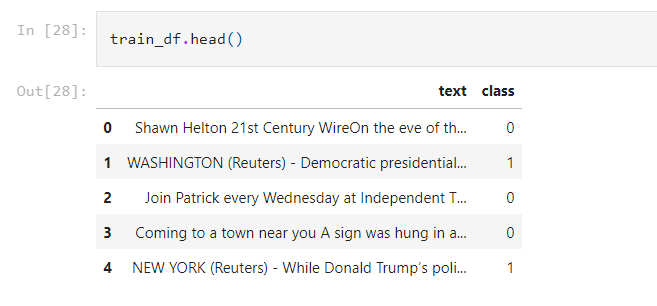
\includegraphics[width=0.98\linewidth]{img/train-csv.PNG}
\caption{Tập train, có gán nhãn}
\end{figure}

\column{.5\textwidth}
\begin{figure}
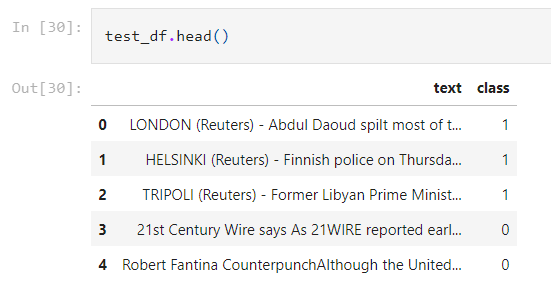
\includegraphics[width=0.9\linewidth]{img/test-csv.PNG}
\caption{Tập test, có gán nhãn}
\end{figure}
\end{columns}
\end{frame}

\begin{frame}{Preprocessing (cont.)}
\begin{columns}[c]

\column{.4\textwidth}
\begin{block}{Trước}
LONDON (Reuters) - Abdul Daoud spilt most of the cappuccino into the saucer the first time he served Princess Diana, his nerves getting the better of him. Almost 20 years on since she was killed when her car crashed in a Paris tunnel, he still works surrounded by pictures of the woman he calls "the princess of the people" in his cafe, named Diana, his very personal attempt to keep her memory alive.
\end{block}
\pause
\column{.4\textwidth}
\begin{block}{Sau}
london  reuters    abdul daoud spilt most of the cappuccino into the saucer the first time he served princess diana  his nerves getting the better of him  almost  years on since she was killed when her car crashed in a paris tunnel  he still works surrounded by pictures of the woman he calls  the princess of the people  in his cafe  named diana  his very personal attempt to keep her memory alive 
\end{block}
\end{columns}
\end{frame}

\begin{frame}
	\Huge{\centerline{\textbf{Feature Extraction}}}
\end{frame}

\begin{frame}{Feature Extraction}
\begin{itemize}
\item Ta không `học thuộc` một câu, mà chỉ `học` những gì đặc trưng của câu đó.
\item Có nhiều cách trích xuất đặc trưng của câu: TF-IDF, BoW (đánh trọng số); GloVe, Word2Vec (chuyển câu thành dạng vector)
\item Một cách làm `tầm thường`: tính tần suất xuất hiện của những từ trong câu (trong đoạn văn / bài viết) và dựa trên tần suất lựa chọn các từ đặc trưng (TF).
\end{itemize}
\end{frame}

\begin{frame}{Feature Extraction - TF-IDF}
\begin{itemize}
\item Term Frequency - Inverse Document Frequency
\item Phương pháp này làm giảm ảnh hưởng của những từ thường xuyên xuất hiện trong corpus.
\item Công thức biểu diễn trọng số $W$ của một từ (term) $t$ trong văn bản (document) $d$:
$$
W(d, t) = TF(d, t) \times \log\left(\frac{N}{df(t)}\right)
$$
Với $N$ là tổng số document, $df(t)$ là số lượng document chứa term $t$. $TF(d, t)$ là số lần xuất hiện của từ $t$ trong document $d$.
\end{itemize}
\end{frame}

\subsection{Decision Tree}

\begin{frame}
	\Huge{\centerline{\textbf{Decision Tree (Cây Quyết định)}}}
\end{frame}

\begin{frame}{Decision Tree}
Nhắc lại:
\begin{itemize}
\item Được Ross Quinlan sáng tạo năm 1986\cite{DBLP:journals/ml/Quinlan86}, là phương pháp xuất hiện từ rất sớm và rất thành công trong nhiều lĩnh vực của text classification.
\item Có nhiều phiên bản: ID3, ID4.5, ID5.0, CART\footnote{sklearn.tree.DecisionTreeClassifier sử dụng phiên bản customize của thuật CART}
\item Ý tưởng: tạo một cấu trúc dữ liệu cây, mỗi nút lá là một thuộc tính của tập dữ liệu đã phân lớp; mỗi nút không phải nút lá biểu thị một phép thử với một thuộc tính; mỗi nhánh biểu thị kết quả của phép thử.
\end{itemize}
\end{frame}

\begin{frame}{Decision Tree (cont.) - Ví dụ}
\centering{
\begin{forest}
[Hết kem đánh răng?, tikz={\draw[{Latex}-, thick] (.north) --++ (0,1);}
	[Trời mưa?,edge label={node[midway,left] {\small{Hết}}} 
		[Ở nhà, edge label={node[midway,left] {\small{Đang mưa}}}]
		[Đi mua, edge label={node[midway,right] {\small{Không mưa}}}] 
	]
	[Ở nhà, edge label={node[midway,right] {\small{Chưa hết}}}
	]   
] 
\end{forest}
}

\begin{itemize}
	\item Q: Làm sao biết thuộc tính nào là nút cha, thuộc tính nào là nút con?
	\item A: Feature Selection, có thể sử dụng độ đo Information Gains (IG) hoặc Gini Index.
\end{itemize}
\end{frame}

\begin{frame}{Decision Tree (cont.) - Feature Selection with IG}
\begin{itemize}
\item Hàm số Entropy:
$$
H(\textbf{p}) = -\sum_{i = 1}^n p_i\log(p_i)
$$
Với $\textbf{p} = (p_1, p_2, .., p_n)$ là phân phối sao cho biến ngẫu nhiên $x$ nhận $n$ giá trị $(x_1, x_2, .., x_n)$ và xác suất lần lượt là $(p_1, p_2, .., p_n)$.

\begin{itemize}
\item Ví dụ: một tập dữ liệu có $p$ samples được gán nhãn \textit{positive} và $n$ samples được gán nhãn \textit{negative}. Khi đó entropy $H(\frac{p}{n + p}, \frac{n}{n + p})$ được tính như sau:
$$
H\left(\frac{p}{n + p}, \frac{n}{n + p}\right) = - \frac{p}{n + p}\log\left(\frac{p}{n + p}\right) - \frac{n}{n + p}\log\left(\frac{n}{n + p}\right)
$$
\end{itemize}
\end{itemize}
\end{frame}

\begin{frame}{Decision Tree (cont.) - Feature Selection with IG}
\begin{itemize}
\item Chọn thuộc tính $A$ có $k$ giá trị khác nhau, chia tập train $E$ thành các tập con $\{E_1, E_2, .., E_k\}$. \textbf{Entropy kỳ vọng (EH)} còn lại sau khi chọn $A$ là một nút:
$$
EH(A) = \sum_{i = 1}^{k} \frac{p_i + n_i}{p + n} H\left(\frac{p_i}{n_i + p_i}, \frac{n_i}{n_i + p_i}\right)
$$
\item Độ đo \textbf{Information Gains}:
$$
A(I) = H\left(\frac{p}{n + p}, \frac{n}{n + p}\right) - EH(A)
$$
Ta sẽ chọn thuộc tính có Information Gain lớn nhất làm nút cha.
\end{itemize}
\end{frame}

\begin{frame}{Decision Tree (cont.) - so sánh}
    \begin{figure}
        \centering
        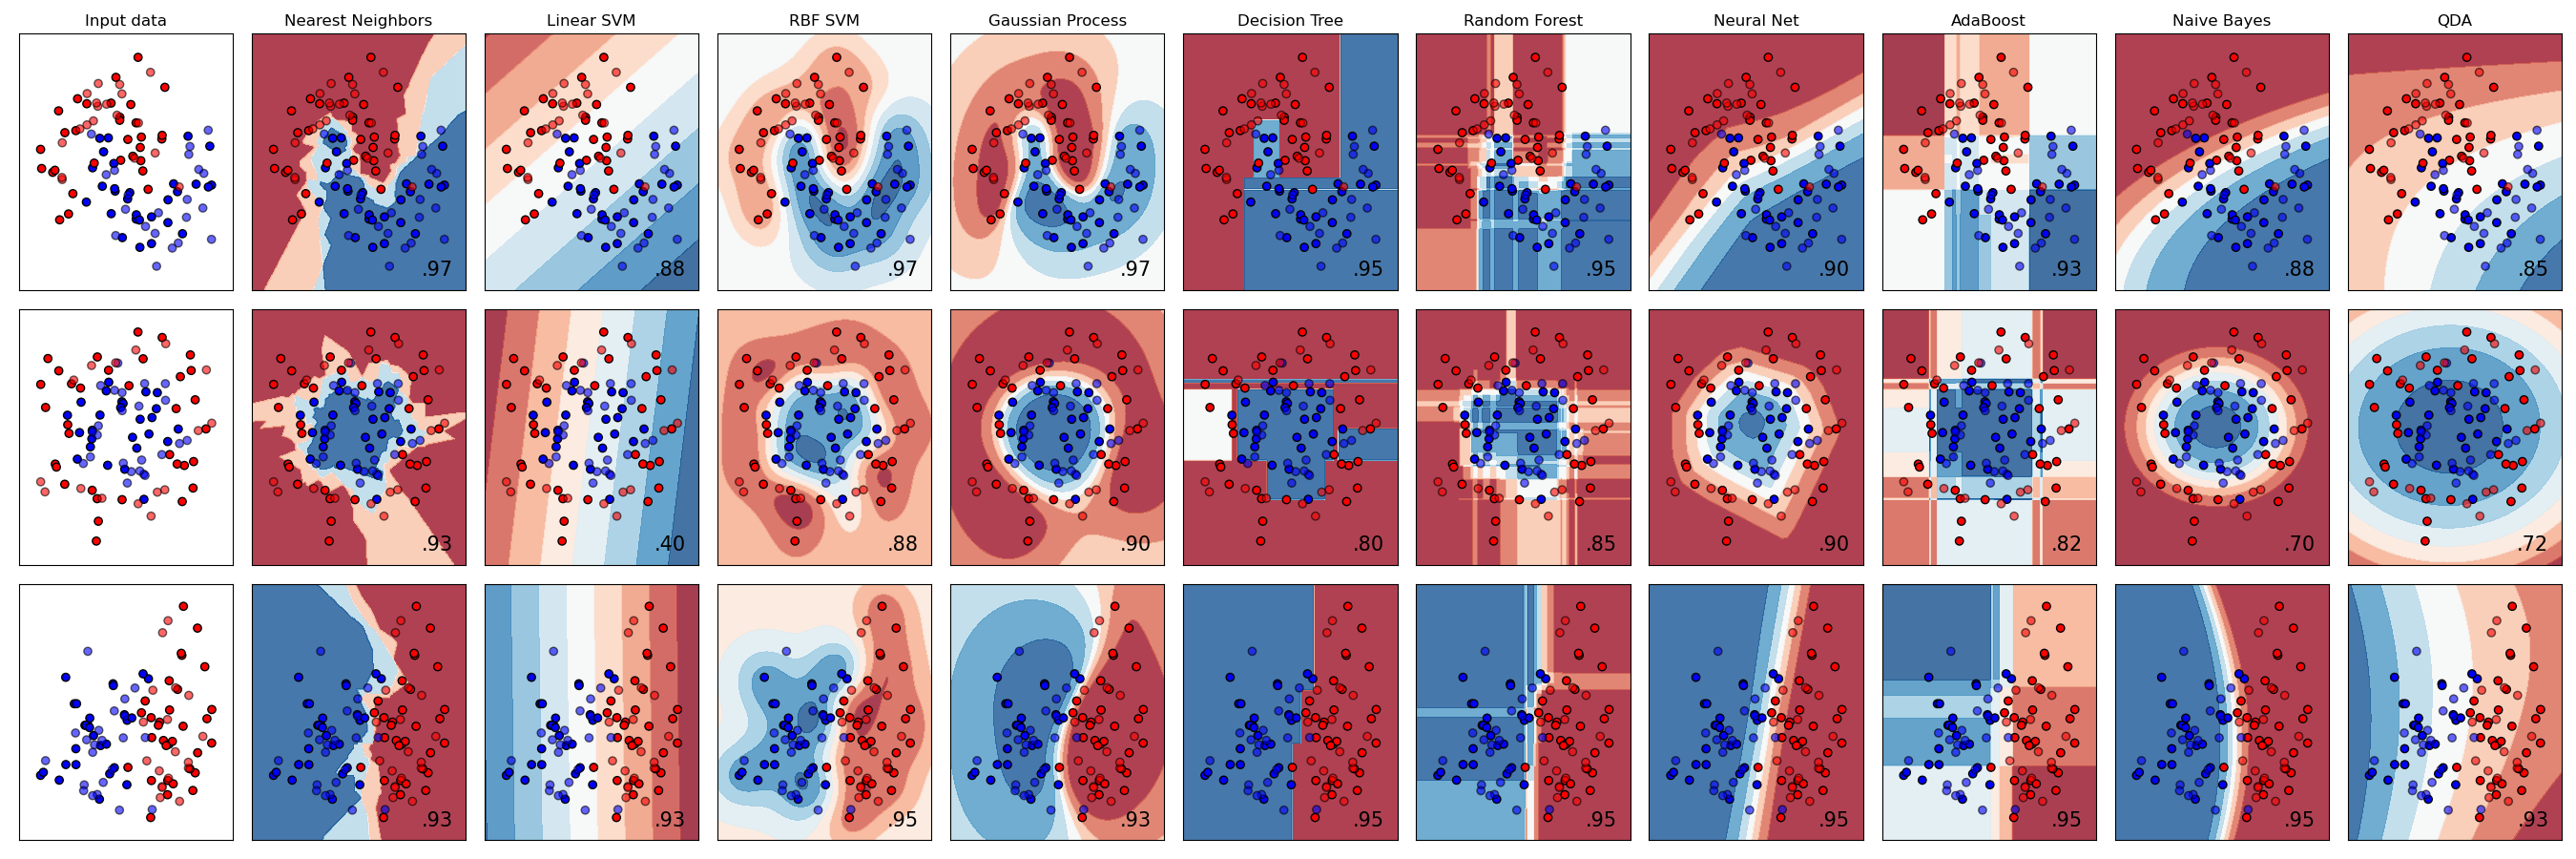
\includegraphics[scale=.2]{img/classifiers-comparison.png}
        \caption{So sánh các classifier, nguồn \cite{scikit-learn}}
    \end{figure}
\end{frame}

\subsection{Training \& testing}

\begin{frame}
	\Huge{\centerline{\textbf{Training \& Testing}}}
\end{frame}

\begin{frame}{Training \& testing}
\begin{figure}
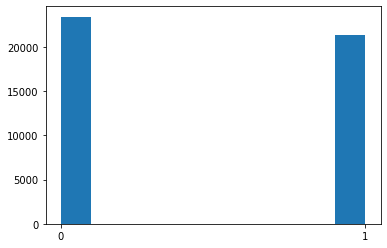
\includegraphics[width=0.35\linewidth]{img/real-fake-in-train.png}
\caption{Tương quan các lớp fake (0) và real (1) trong tập train}
\end{figure}

\begin{itemize}
\item Kích thước tập train: 44798 samples, gồm các articles đã được gán nhãn 0 (fake) và 1 (real).
\item Kích thước tập test: 100 samples, gồm 50 article được chọn ngẫu nhiên từ tập real + 50 article được chọn ngẫu nhiên từ tập fake.
\item Sử dụng \texttt{sklearn.tree.DecisionTreeClassifier}.
\end{itemize}
\end{frame}

\begin{frame}{Training \& testing (cont.)}
\begin{columns}[c]
\column{.35\textwidth}
\begin{figure}
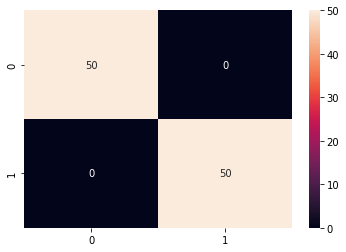
\includegraphics[width=0.8\linewidth]{img/train-result.png}
\caption{Heatmap kết quả testing}
\end{figure}
\column{.65\textwidth}
\begin{table}
\begin{tabular}{l l l l l}
\toprule
 & precision & recall & f1-score & support \\
\midrule
0 & 1.00 & 1.00 & 1.00 & 50 \\
1 & 1.00 & 1.00 & 1.00 & 50 \\
accuracy &   &   & 1.00 & 100 \\
macro avg & 1.00 & 1.00 & 1.00 & 100 \\
weighted avg & 1.00 & 1.00 & 1.00 & 100 \\
\bottomrule
\end{tabular}
\caption{\texttt{classification\_report} sau khi train}
\end{table}
\end{columns}
Nhận xét: 
\begin{itemize}
    \item Độ chính xác gần như tuyệt đối (1.00).
    \item Thời gian train rất nhanh.
\end{itemize}
\end{frame}

\section{Demo}
\begin{frame}{Demo}
    \Huge{\centerline{\textbf{Xem demo trực tiếp..}}}
\end{frame}

\begin{frame}{Tổng kết}
Ưu điểm:
\begin{itemize}
\item Decision Tree là thuật toán phân lớp phổ biến, dễ cài đặt.
\item Cho độ chính xác cao với tập dữ liệu nhỏ.
\item Thời gian huấn luyện nhanh.
\end{itemize}
Khuyết điểm:
\begin{itemize}
\item Dễ bị overfit. Xử lý: pruning.
\item `Nhạy cảm` với sự xáo trộn dữ liệu.\cite{Kowsari_2019}
\begin{itemize}
	\item "Thử" xài nltk.stop\_word thay cho english stopwords của TfidfVectorizer?
\end{itemize}
\end{itemize}
\end{frame}

\begin{frame}
    \Huge{\centerline{\textbf{QnA}}}
\end{frame}

\section{Tài liệu}

\begin{frame}{Tài liệu}
    \printbibliography
\end{frame}

\begin{frame}
    \Huge{\centerline{\textbf{Fin}}}
\end{frame}

\end{document}